% !TEX root = 0000.tex
% Capítulo 3: Experimentation and Results
% Contenido tomado de main_2.tex (líneas 2623-3212) sin cambios de texto.

% El texto está en inglés: reglas de corte de palabra del inglés
\begin{hyphenrules}{english}

\chapter{Experimentation and Results}\label{ch:experiments}

This chapter evaluates the architectures of Chapter~\ref{ch:pinns} along two complementary lines. The first
one is a controlled case study, the linear homogeneous Klein--Gordon equation (Section~\ref{sec:klein-gordon}),
where the reference solution is exact in time and the number of frequencies of the initial condition can
be controlled; it contains a preliminary optimization experiment (Section~\ref{sec:exp-preliminary}), the
comparison of architectures (Section~\ref{sec:exp-architectures}) and a study of regularization and of the
Fourier scale (Section~\ref{sec:exp-regularization}). The second line is breadth: MABUR-PINN is evaluated on
twelve tasks of the PINNacle benchmark, which contain elliptic, parabolic and hyperbolic equations
(Section~\ref{sec:exp-benchmark}). Section~\ref{sec:exp-synthesis} relates the results with the theory of
Chapters~\ref{ch:pdes} and \ref{ch:pinns}.

% =====================================================================
\section{General Methodology}\label{sec:exp-methodology}
% =====================================================================

\paragraph{Metrics.}
For all experiments we report the relative $L^2$ error on a reference grid of
$N_{\mathrm{test}}$ points $(\mathbf{x}_j,t_j)$,
\begin{equation}
  \mathrm{L2RE}=\frac{\big(\sum_j\abs{u_\theta(\mathbf{x}_j,t_j)-u(\mathbf{x}_j,t_j)}^2\big)^{1/2}}{\big(\sum_j\abs{u(\mathbf{x}_j,t_j)}^2\big)^{1/2}},
  \label{eq:l2re}
\end{equation}
which is the discrete version of the total error $\mathcal{E}(\theta)$ of Section~\ref{sec:pinn-formulation};
the mean absolute error; the number of trainable parameters; and the final value of the (weighted)
loss, which is the training error $\mathcal{E}_T^2$. Reporting both the loss and the L2RE is important,
because Theorem~\ref{thm:error-decomp} says that they are different things.

\paragraph{Implementation.}
All networks were implemented and trained by us under the same conditions. We used mixed precision:
32-bit floating point only for the parameters of the network, and 64-bit floating point for the
collocation points, the optimization coefficients, the back-propagated gradients, etc. The code and the
results are available in the repositories
\url{https://github.com/Emmaquantum/HPINN} and \url{https://github.com/Emmaquantum/Optimization_PINN}.
\verificar{framework (PyTorch/JAX), hardware (GPU), training time and number of random seeds per
configuration}

% =====================================================================
\section{Reference Solution: Pseudo-Spectral Propagator}\label{sec:reference-solution}
% =====================================================================

\paragraph{Problem.}
We consider the one-dimensional Klein--Gordon equation \eqref{eq:kg} in natural units ($m=c=\hbar=1$):
\begin{equation}
  \begin{cases}
    \partial_{tt}\phi(x,t)-\partial_{xx}\phi(x,t)+m^2\phi(x,t)=0, & x\in\Omega=[-L/2,L/2],\ t\in[0,T],\\
    \phi(-L/2,t)=\phi(L/2,t), & t\in[0,T],\\
    \phi(x,0)=A\exp\Big(-\dfrac{x^2}{2\sigma^2}\Big)\displaystyle\sum_{k\in\mathcal{K}}\big(e^{ikx}+e^{-ikx}\big), & x\in\Omega,\\
    \partial_t\phi(x,0)=0, & x\in\Omega.
  \end{cases}
  \label{eq:kg-problem}
\end{equation}
The initial conditions represent a stationary particle, that is, a localized pulse with zero initial
velocity. The initial position is a Gaussian envelope modulated by a symmetric phase, which induces
velocity in $+k$ and $-k$. This initial condition can be manipulated consciously so that the network
needs to learn high and low frequencies at the same time, by introducing a set of wavenumbers
$\mathcal{K}=\{k_1,k_2,\dots,k_n\}$ with $k_1<k_2<\dots<k_n$. Because of the dispersion relation
Equation~\eqref{eq:kg-dispersion}, each wavenumber travels with a different group velocity: the pulse disperses
inside the light cone $\abs{x}\le t$. The boundary condition is periodic, as required by the
pseudo-spectral method; however, with the chosen parameters the wave does not reach the boundary during
the simulation. In Experiment~1 we use $\mathcal{K}=\{1,5,10\}$, $\sigma=1$, $L=80$ and $T=36$.
\verificar{value of the amplitude $A$; the presentation writes $\Omega=[-L,L]$ but the figures show
$x\in[-40,40]$}

\paragraph{Choice of parameters.}
The solution of Equation~\eqref{eq:kg-problem} models the field of a free particle released into an (almost)
infinite space. To achieve this, the space must be large enough to model an infinite space, $L\gg\sigma$,
and the simulation time must be short enough so that the wave does not hit the boundary.
\begin{enumerate}
  \item \textbf{Space:} $L\ge40\sigma$, enough times $\sigma$ so that the boundary is not reached.
  \item \textbf{Time:} since the group velocity is bounded by $c=1$ (Equation~\eqref{eq:kg-group-velocity}), the
    fastest front reaches the boundary at $t=L/2$. The thickness of the pulse is about $4\sigma$, so we
    take $T\approx L/2-4\sigma$; for $L=80$ and $\sigma=1$, $T=36$.
  \item \textbf{Grid:} in a classical explicit scheme we would need the CFL (Courant--Friedrichs--Lewy)
    condition $c\,\Delta t/\Delta x\le1$. Here the propagator is exact in time, so the scheme is
    unconditionally stable, and the time step only defines the temporal resolution of the stored
    solution. What matters is that the spatial grid resolves the largest wavenumber of the initial
    condition: with $N$ grid points, $\Delta x=L/N$ and we need $k_{\max}<\pi/\Delta x$. With $N=1000$ and
    $L=80$, $\pi/\Delta x\approx39>k_{\max}=10$.\verificar{whether $N=1000$ is the number of spatial points
    or of time steps}
\end{enumerate}

\paragraph{Propagator.}
The solution is exact in Fourier space, which means that, by means of a propagator
\cite{hochbruck2010}, the solution is computed without numerical errors beyond the truncation of the
Fourier series; all we have to do is to compute the propagator and iterate. With the change of variables
$v=\partial_t\phi$ and the operator $\mathcal{L}=m^2-\partial_{xx}$, the Klein--Gordon equation becomes
the first-order system
\begin{equation}
  \frac{\,d}{\,d t}\begin{pmatrix}\phi\\ v\end{pmatrix}
  =\underbrace{\begin{pmatrix}0 & 1\\ -\mathcal{L} & 0\end{pmatrix}}_{A}
  \begin{pmatrix}\phi\\ v\end{pmatrix},
  \qquad\mathbf{y}(t)=e^{At}\mathbf{y}(0),
  \label{eq:kg-first-order}
\end{equation}
with $\mathbf{y}=(\phi,\partial_t\phi)^{T}$. The propagator $e^{At}$ is responsible for the temporal
evolution of the field. Expanding it in Taylor series and separating the even and odd powers of $A$
(Appendix~\ref{app-sec:kg-propagator}), we obtain
\begin{equation}
  e^{At}=\begin{pmatrix}
    \cos\big(t\sqrt{\mathcal{L}}\big) & \dfrac{\sin(t\sqrt{\mathcal{L}})}{\sqrt{\mathcal{L}}}\\[2mm]
    -\sqrt{\mathcal{L}}\sin\big(t\sqrt{\mathcal{L}}\big) & \cos\big(t\sqrt{\mathcal{L}}\big)
  \end{pmatrix}.
  \label{eq:kg-propagator}
\end{equation}
To evaluate the
operator $\mathcal{L}$ numerically we take advantage of the periodic boundary condition: the Fourier
transform diagonalizes it, $\widehat{\mathcal{L}}=m^2-(ik)^2=m^2+k^2=\omega_k^2$, and the propagator becomes
a $2\times2$ rotation for each wavenumber:
\begin{equation}
  \begin{pmatrix}\hat\phi_k(t)\\ \hat{\dot\phi}_k(t)\end{pmatrix}
  =\begin{pmatrix}
    \cos(\omega_kt) & \dfrac{\sin(\omega_kt)}{\omega_k}\\[2mm]
    -\omega_k\sin(\omega_kt) & \cos(\omega_kt)
  \end{pmatrix}
  \begin{pmatrix}\hat\phi_k(0)\\ \hat{\dot\phi}_k(0)\end{pmatrix}.
  \label{eq:kg-propagator-fourier}
\end{equation}
This is exactly the discrete version of the exact solution \eqref{eq:kg-fourier-solution}. The algorithm
is Algorithm~\ref{alg:pseudospectral}.

\begin{algorithm}[htbp]
  \caption{Pseudo-spectral method for the Klein--Gordon equation.}
  \label{alg:pseudospectral}
  \begin{algorithmic}[1]
    \Require Physical parameters $m$, $L$, $T$, $N$; initial conditions $\phi(x,0)$, $\dot\phi(x,0)$.
    \State $\Delta x\gets L/N$, $\Delta t\gets T/N_t$ \Comment{precomputation of the frequency space}
    \State $k\gets 2\pi\cdot\texttt{fftfreq}(N,\Delta x)$; \quad $\omega_k\gets\sqrt{m^2+k^2}$
    \State $\hat\phi_k\gets\mathrm{FFT}(\phi(x,0))$; \quad $\hat{\dot\phi}_k\gets\mathrm{FFT}(\dot\phi(x,0))$ \Comment{initial transform}
    \State $C_k\gets\cos(\omega_k\Delta t)$; \quad $S_k\gets\sin(\omega_k\Delta t)$
    \State $t\gets0$
    \While{$t<T$} \Comment{time evolution, Equation~\eqref{eq:kg-propagator-fourier}}
      \State $\hat\phi^{\mathrm{new}}_k\gets C_k\hat\phi_k+\frac{1}{\omega_k}S_k\hat{\dot\phi}_k$
      \State $\hat{\dot\phi}^{\mathrm{new}}_k\gets-\omega_kS_k\hat\phi_k+C_k\hat{\dot\phi}_k$
      \State $\hat\phi_k\gets\hat\phi^{\mathrm{new}}_k$; \quad $\hat{\dot\phi}_k\gets\hat{\dot\phi}^{\mathrm{new}}_k$; \quad $t\gets t+\Delta t$
      \State store $\phi(x,t)\gets\operatorname{Re}\big(\mathrm{IFFT}(\hat\phi_k)\big)$ \Comment{recovery to real space}
    \EndWhile
    \State \Return history $\phi(x,t)$
  \end{algorithmic}
\end{algorithm}

Figure~\ref{fig:ps-evolution} shows the initial condition and the evolution of the field used in the
preliminary experiment. The field disperses inside a light cone, at the same velocity to the left and
to the right.

\begin{figure}[htbp]
  \centering
  \begin{subfigure}[b]{0.36\linewidth}
    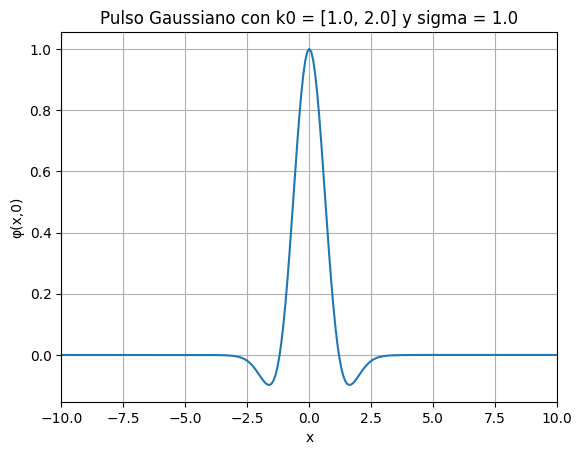
\includegraphics[width=\linewidth]{ic_gaussian.png}
    \caption{Initial condition (Gaussian pulse).}
  \end{subfigure}\hfill
  \begin{subfigure}[b]{0.62\linewidth}
    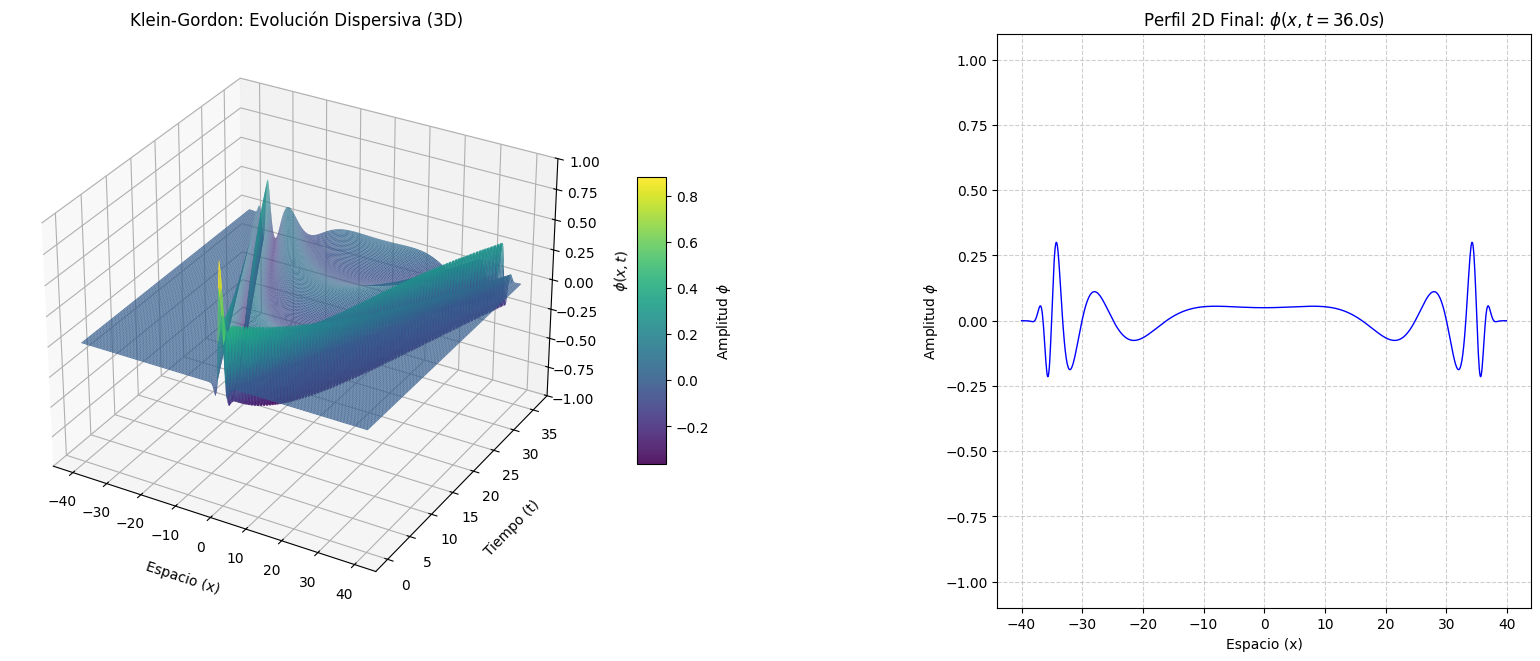
\includegraphics[width=\linewidth]{ps_evolution.png}
    \caption{Evolution of the field and final profile.}
  \end{subfigure}
  \caption[Pseudo-spectral reference solution of the preliminary experiment]{Pseudo-spectral reference solution of the preliminary experiment. (a) Initial condition,
  Gaussian with $\sigma=1$. (b) Evolution of the field during $36$ time units: the field disperses
  inside a light cone at the same velocity to the left and to the right, and the final profile shows
  the dispersion of the pulse once released in the (almost) infinite domain. A video of the evolution is
  available in the repository.}
  \label{fig:ps-evolution}
\end{figure}
\verificar{the text of the first report says $k_0=0.5$, but the title of panel (a) says $k_0=[1,2]$}

% =====================================================================
\section{Preliminary Experiment: ADAM + LRA and L-BFGS}\label{sec:exp-preliminary}
% =====================================================================

The first experiment asks a simple question: how well can a PINN with a periodic activation, trained with
the strategies of Section~\ref{sec:gradient-pathologies}, reproduce the dispersion of a static spin-0 particle?
We used a SIREN network ($\omega_0=30$) with $128$ neurons per hidden layer and $6$ hidden layers; this
architecture was obtained by experimentation until a good performance was reached. We used ADAM + LRA as a
first stage to characterize the minima within the set of achievable values: exponential decay of the
learning rate with $\eta_0=10^{-4}$ and rate $0.95$ every $1\,500$ iterations; the weights of the initial
and boundary losses were recomputed every $10$ iterations and updated with a moving average with
$\alpha=0.95$, starting from $(1,1,1)$. A random sampling algorithm generated new points
$(\mathbf{x}_i,t_i)$, $i\in\{f,ic,bc\}$, at each iteration \cite{wang2021gradient,liu2022}, starting from $128$
collocation points for each loss term; in this way, after $50\,000$ iterations the network was trained
with a total of $6.4$ million collocation points without saturating the memory.\verificar{the report
mentions both $50\,000$ and $100\,000$ ADAM iterations} After ADAM + LRA found a region where the
optimal value is, a variant of L-BFGS was used as final minimizer, with a stopping criterion of $5\,000$
iterations or a tolerance of machine epsilon; the weights and parameters of the first stage were loaded as
initialization, so that the second stage has some ``memory'' of the first one. The physical conditions
were the same as in the numerical simulation.

\paragraph{Results.}
The optimizer ADAM + LRA reduced the total loss to orders of $10^{-5}$ after the training, with a final
learning rate of $\approx3.27\times10^{-6}$ and final weights $(1.0,\,4.90,\,0.82)$, reaching stability at
a Pareto value (Figure~\ref{fig:prelim-loss}a). Although there seems to be convergence, ADAM is slow when
converging to minima, but fast approaching them when the gradients are balanced; since they are not, LRA
was used, and the curve shows a lot of noise produced by the change of weights every $10$ epochs. The
SIREN method favors the boundary conditions, so the boundary loss can reach values close to $10^{-12}$; the
total loss remained in the hands of the physics (PDE) loss and the initial condition.

The second-order optimizer L-BFGS refined the solution, reaching a total loss of order $10^{-8}$
(Figure~\ref{fig:prelim-loss}b), with smooth curves, no numerical explosions, and convergence in fewer than
$500$ iterations, which indicates that the inherited weights were good enough for the optimizer to reach
an almost even convergence of all the loss terms. The PDE loss converged rapidly, indicating strong
learning of the Klein--Gordon equation, that is, the network learned not to violate the physical law.

\begin{figure}[htbp]
  \centering
  \begin{subfigure}[b]{0.49\linewidth}
    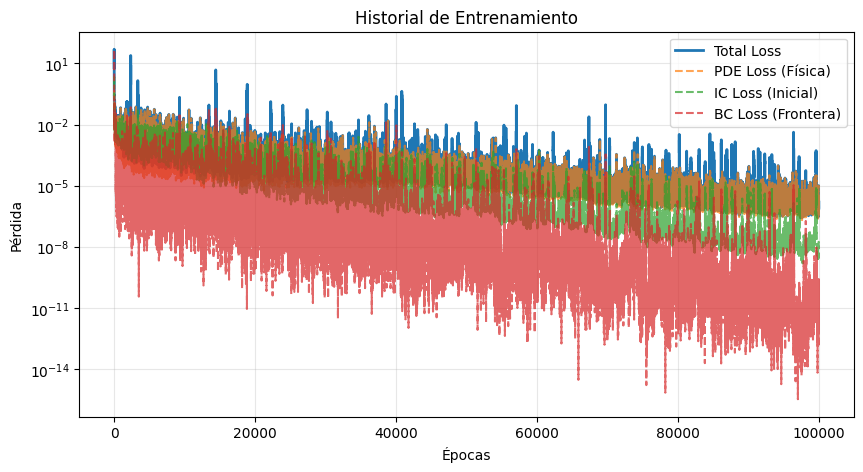
\includegraphics[width=\linewidth]{prelim_adam_loss.png}
    \caption{ADAM + LRA.}
  \end{subfigure}\hfill
  \begin{subfigure}[b]{0.49\linewidth}
    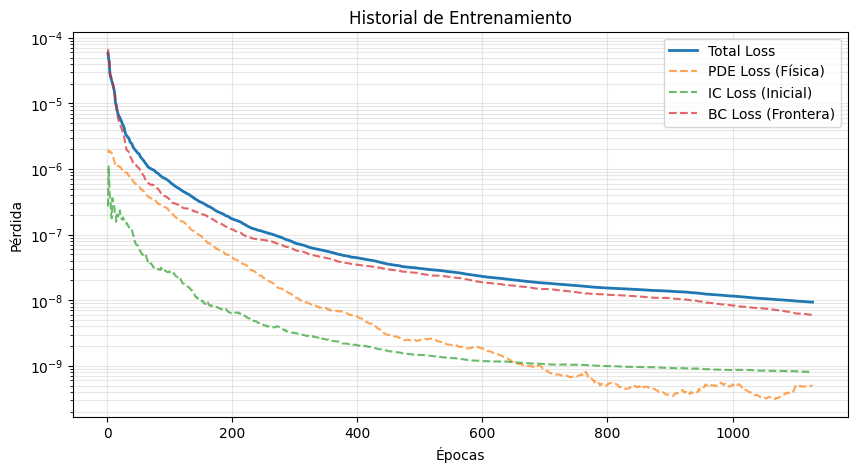
\includegraphics[width=\linewidth]{prelim_lbfgs_loss.png}
    \caption{L-BFGS.}
  \end{subfigure}
  \caption[Loss functions through the training epochs of the preliminary experiment]{Loss functions through the training epochs of the preliminary experiment. (a) ADAM + LRA:
  the noise comes from the update of the weights every $10$ epochs. (b) L-BFGS: smooth curves, without
  numerical explosions.}
  \label{fig:prelim-loss}
\end{figure}

Although the network learned the initial condition (Gaussian pulse) very well
(Figure~\ref{fig:prelim-validation}a), the validation against the numerical simulation shows conflicts: the
relative $L^2$ error is $9.53\%$ (Figure~\ref{fig:prelim-validation}b). The PINN generates the cone of the group
velocity of the fastest waves (inside the light cone), but it is still inconsistent in amplitude. We
interpret this result as an apparent Pareto value \cite{rohrhofer2023}: a training loss of order
$10^{-8}$ together with an error of almost $10\%$. In the language of Theorem~\ref{thm:error-decomp}, the training
error is small, but the generalization gap and the approximation error are not; this observation motivated
the comparison of architectures of the next section.

\begin{figure}[htbp]
  \centering
  \begin{subfigure}[b]{0.34\linewidth}
    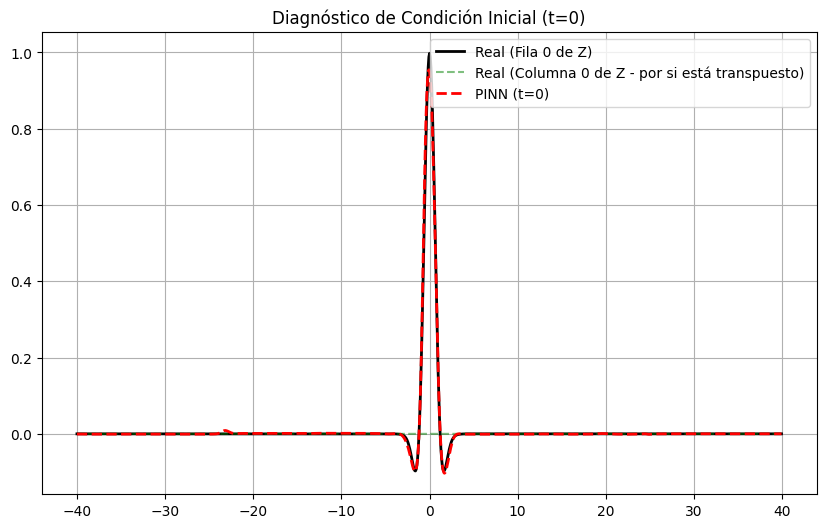
\includegraphics[width=\linewidth]{prelim_ic_diagnostic.png}
    \caption{Initial condition ($t=0$).}
  \end{subfigure}\hfill
  \begin{subfigure}[b]{0.64\linewidth}
    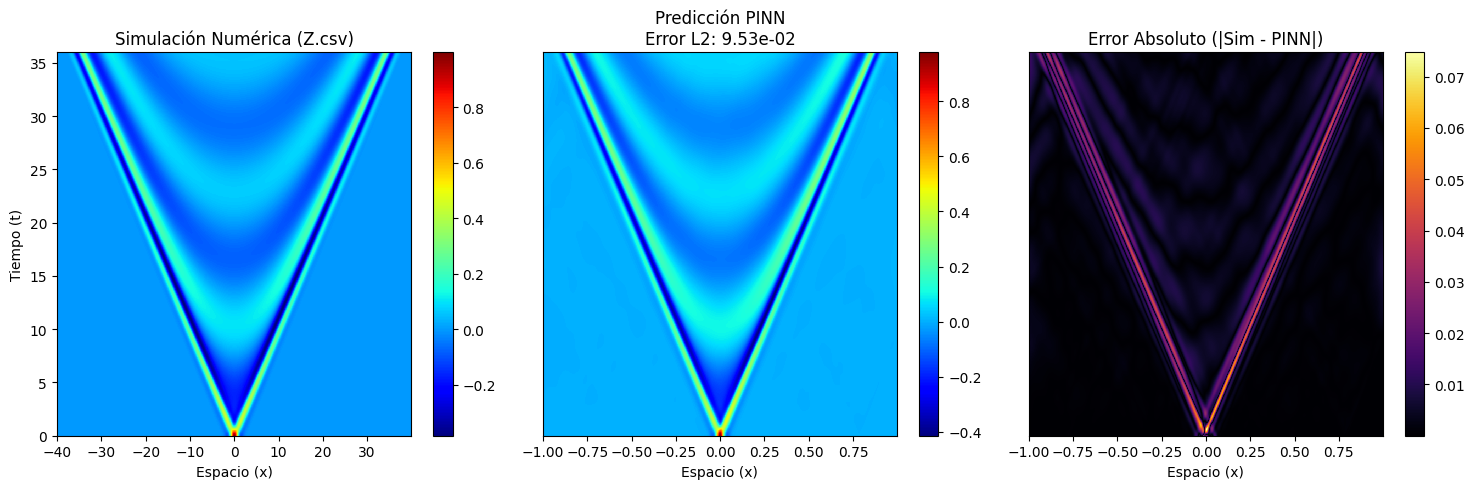
\includegraphics[width=\linewidth]{prelim_comparison.png}
    \caption{Simulation, PINN prediction and absolute error.}
  \end{subfigure}
  \caption[Validation of the preliminary experiment]{Validation of the preliminary experiment. (a) The network fits the static behavior at
  $t=0$ very well. (b) The PINN reproduces the light cone, but the amplitude inside the cone is still
  inconsistent (L2RE $=9.53\%$).}
  \label{fig:prelim-validation}
\end{figure}

% =====================================================================
\section{Experiment 1: Comparison of Architectures}\label{sec:exp-architectures}
% =====================================================================

\paragraph{Methodology.}
We replicated each of the architectures of Section~\ref{sec:architectures} and implemented them on the
Klein--Gordon problem \eqref{eq:kg-problem} with $\mathcal{K}=\{1,5,10\}$, to analyze their behavior. All
the networks were trained with the same strategies: input scaling (Equation~\eqref{eq:normalization}), learning rate
annealing (Section~\ref{subsec:lra}), causal training (Equation~\eqref{eq:causal}), focused stochastic sampling, exponential
decay of the learning rate and mixed precision. The shared configuration is given in
Table~\ref{tab:exp1-config}, and the specific settings of each architecture in Table~\ref{tab:exp1-architectures}.

\begin{table}[htbp]
  \centering
  \caption{Shared training configuration of Experiment~1.}
  \label{tab:exp1-config}
  \small
  \begin{tabular}{@{}ll@{}}
    \toprule
    Component & Configuration \\
    \midrule
    Optimizer & ADAM \cite{kingma2015} \\
    Loss weighting & LRA \cite{wang2021gradient}, $\alpha=0.9$ \\
    Temporal strategy & Causal training \cite{wang2024causality} \\
    Training epochs & $100\,000$ \\
    Learning rate & $10^{-3}$ initial, exponential decay $0.9$ every $2\,000$ epochs \\
    Physics collocation points ($N_f$) & $12\,000$ (80\% inside the light cone) \\
    Initial condition points ($N_{ic}$) & $N_f/2=6\,000$ \\
    Boundary points ($N_{bc}$) & $N_f/4=3\,000$ \\
    Normalization & min--max, $x\in[-1,1]$, $t\in[-1,1]$ \\
    Initial LRA weights & $(1.0,\,1.0,\,0.1)$ \\
    $\omega_0$ (architectures with $\sin$/$\cos$) & $15.0$ (SIREN, AbuPINN, MABUR-PINN) \\
    \bottomrule
  \end{tabular}
\end{table}
\verificar{the presentation reports $t\in[0,1]$ and initial LRA weights $(1,1,1,1)$; unify with the code}

\begin{table}[htbp]
  \centering
  \caption[Architectures of Experiment~1]{Architectures of Experiment~1 ($\epsilon$: causality parameter; chunks: number of temporal
  chunks of the causal loss).}
  \label{tab:exp1-architectures}
  \small
  \begin{tabularx}{\linewidth}{@{}lccccX@{}}
    \toprule
    Architecture & Depth & Width & $\epsilon$ & Chunks & Other \\
    \midrule
    Vanilla \cite{raissi2019} & 6 & 64 & 10 & 16 & $\tanh$ \\
    SIREN \cite{sitzmann2020} & 6 & 64 & 10 & 16 & SIREN activation \\
    MSF \cite{wang2021eigenvector} & 5 & 200 & 10 & 16 & Multiple embedding $\sigma$ \\
    M4 \cite{wang2021gradient} & 6 & 64 & 10 & 16 & Gated architecture + embedding \\
    Abu \cite{wang2023abu} & 6 & 64 & 100 & 16 & Blended activation \\
    MABUR (ours) & 6 (2 bl.) & 64 & 100 & 16 & M4 + Abu + adaptive residual \\
    \bottomrule
  \end{tabularx}
\end{table}

\paragraph{Results.}
Table~\ref{tab:exp1-results} summarizes the results, and Figure~\ref{fig:error-complexity} shows the relative error
against the complexity (number of parameters). MABUR-PINN V2 reaches the lowest error ($1.70\%$ relative
$L^2$) and the lowest final cost ($3.81\times10^{-7}$), followed by AbuPINN ($2.14\%$), which does it with
a moderate number of parameters ($42\,073$), and by M4-PINN ($4.41\%$). In contrast, the vanilla PINN shows
an almost total inability to solve the problem ($71\%$), while MSF-PINN, despite its high number of
parameters ($2.11\times10^{6}$), does not reduce the error significantly ($43.2\%$). MABUR-PINN V1, without
Fourier embedding, reaches $11.2\%$.

\begin{table}[htbp]
  \centering
  \caption{Comparative results of the architectures on the Klein--Gordon equation (Experiment~1).}
  \label{tab:exp1-results}
  \small
  \begin{tabular}{@{}lrrrr@{}}
    \toprule
    Architecture & Rel.\ $L^2$ error (\%) & Abs.\ error & Parameters & Final cost \\
    \midrule
    MABUR-PINN V2 & \textbf{1.70}  & \textbf{0.0006} & 149\,020   & $\mathbf{3.81\times10^{-7}}$ \\
    AbuPINN       & 2.14  & 0.0008 & 42\,073    & $4.60\times10^{-7}$ \\
    M4-PINN       & 4.41  & 0.0013 & 124\,033   & $2.21\times10^{-6}$ \\
    MABUR-PINN V1 & 11.20 & 0.0037 & 51\,177    & $7.25\times10^{-6}$ \\
    PINN-SIREN    & 21.20 & 0.0068 & 21\,057    & $5.85\times10^{-6}$ \\
    MSF-PINN      & 43.20 & 0.0142 & 2\,110\,049 & $9.99\times10^{-5}$ \\
    Vanilla PINN  & 71.00 & 0.0232 & 21\,057    & $6.72\times10^{-5}$ \\
    \bottomrule
  \end{tabular}
\end{table}
\verificar{single run or mean $\pm$ standard deviation over seeds}

\begin{figure}[htbp]
  \centering
  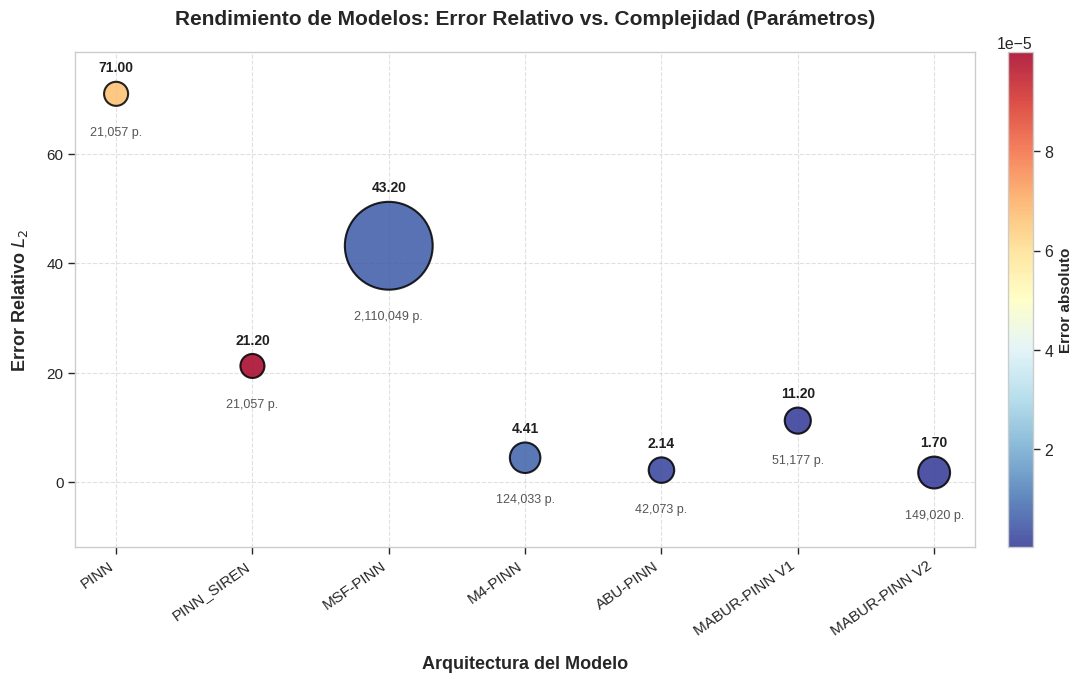
\includegraphics[width=0.85\linewidth]{error_vs_complexity.png}
  \caption[Relative $L^2$ error against complexity]{Relative $L^2$ error (\%) against complexity: the size of each marker is the number of
  parameters and the color is the absolute error.}
  \label{fig:error-complexity}
\end{figure}

Figure~\ref{fig:exp1-maps} compares the error maps of three representative networks; the error maps and loss
curves of all the architectures are in Appendix~\ref{app:figures}. The vanilla PINN has large errors distributed
over the whole cone. AbuPINN has a homogeneous error without pronounced peaks, except near the origin.
MABUR-PINN V2 concentrates its (small) error along the two fronts of the light cone.

\begin{figure}[htbp]
  \centering
  \begin{subfigure}[b]{\linewidth}
    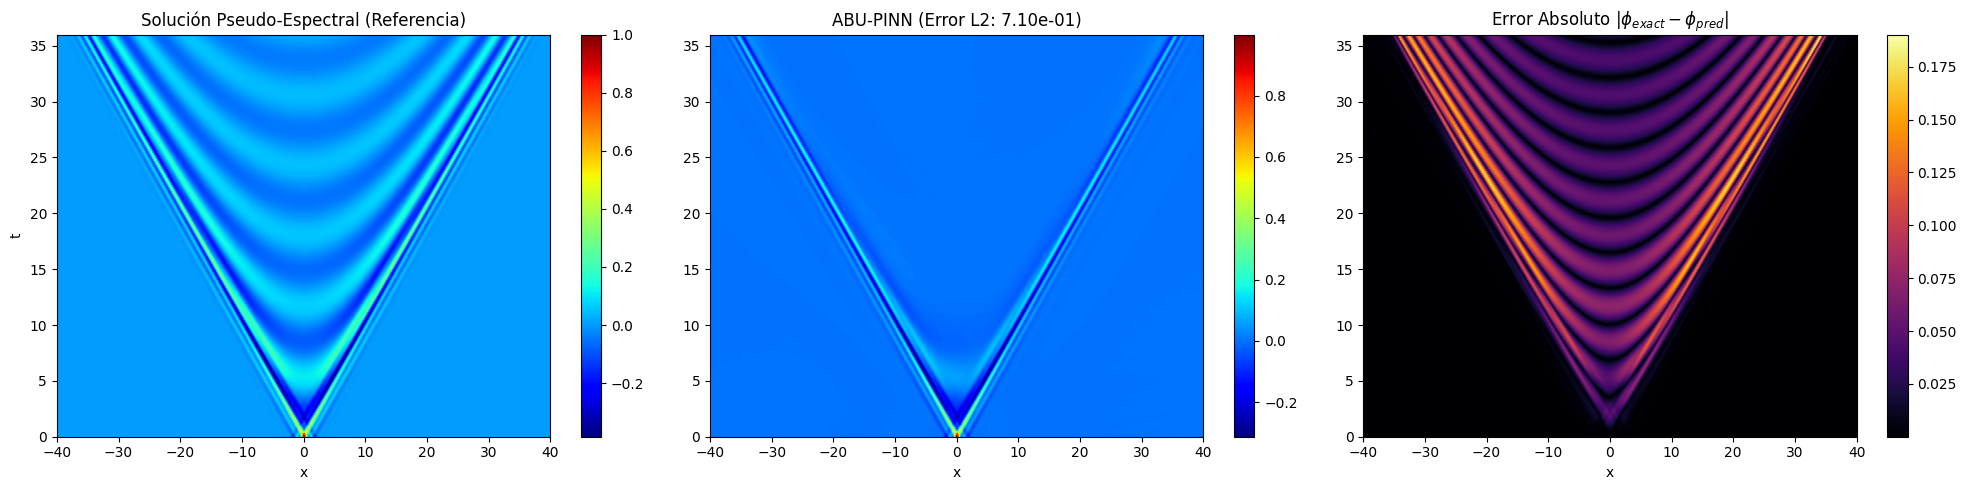
\includegraphics[width=\linewidth]{vanilla_error.png}
    \caption{Vanilla PINN (L2RE $71.0\%$).}
  \end{subfigure}
  \begin{subfigure}[b]{\linewidth}
    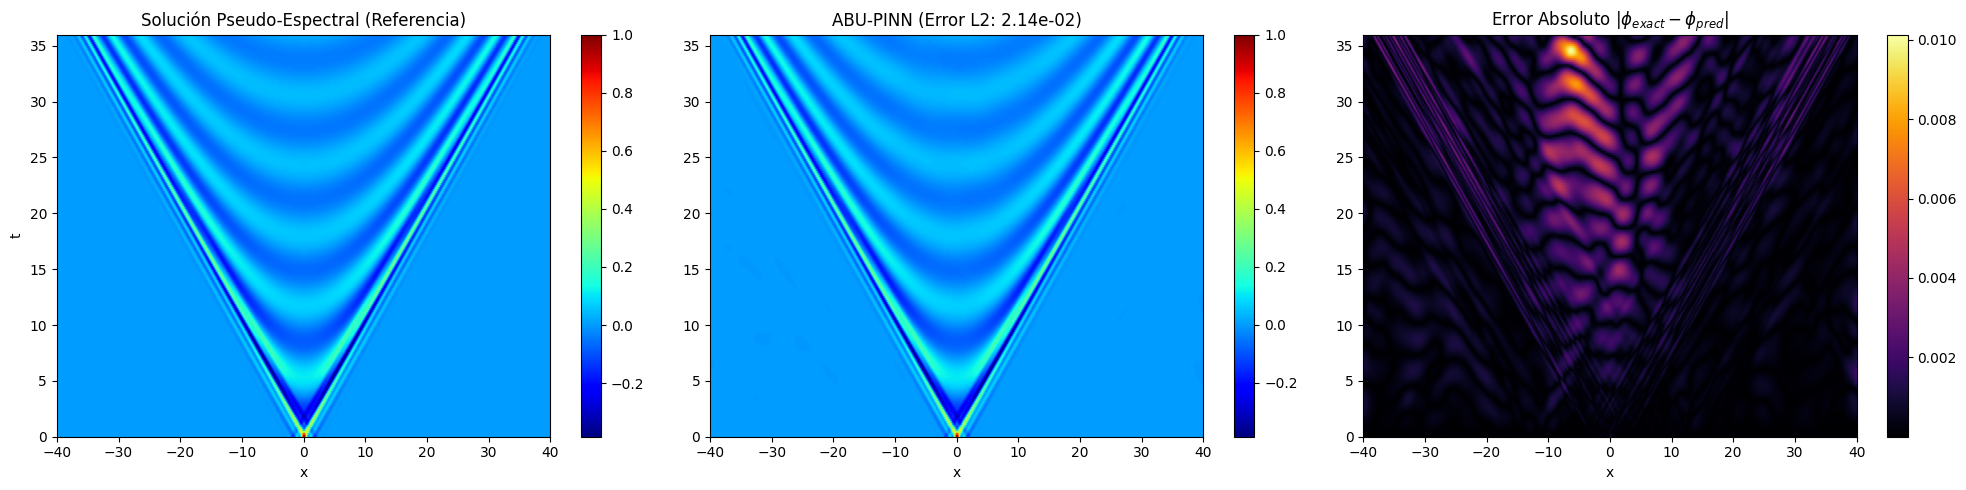
\includegraphics[width=\linewidth]{abu_error.png}
    \caption{AbuPINN (L2RE $2.14\%$).}
  \end{subfigure}
  \begin{subfigure}[b]{\linewidth}
    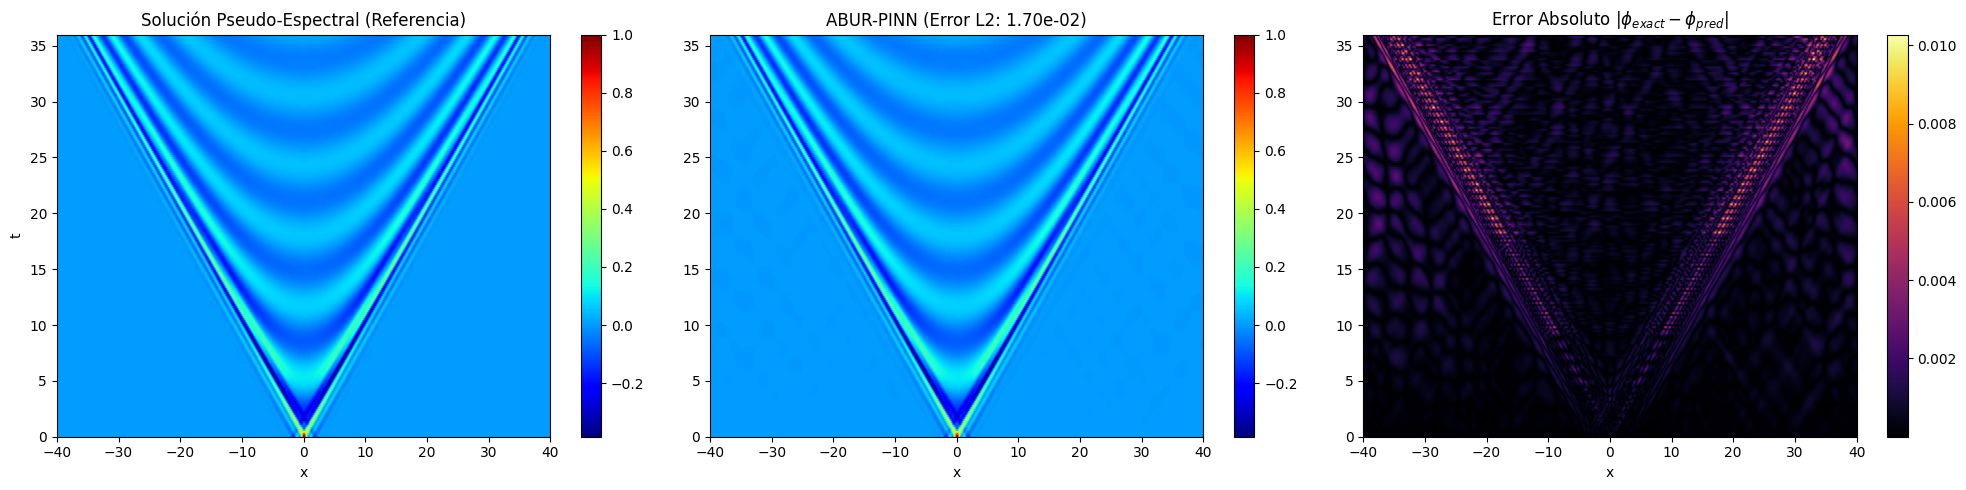
\includegraphics[width=\linewidth]{maburv2_error.png}
    \caption{MABUR-PINN V2 (L2RE $1.70\%$).}
  \end{subfigure}
  \caption[Error maps of three architectures on the Klein--Gordon equation]{Reference solution (left), prediction (center) and absolute error (right) for three
  architectures on the Klein--Gordon equation.}
  \label{fig:exp1-maps}
\end{figure}
\verificar{the panel titles of (a) say ``ABU-PINN'' and those of (c) ``ABUR-PINN''; regenerate the
figures with correct titles, in English}

\paragraph{Discussion.}
Several observations can be extracted.
\begin{enumerate}
  \item \textbf{A low value of the cost function does not guarantee a low relative error.} PINN-SIREN
    reaches a lower final cost than MABUR-PINN V1 ($5.85\times10^{-6}$ vs.\ $7.25\times10^{-6}$), and its
    boundary loss reaches $10^{-12}$, but its error is almost twice as large ($21.2\%$ vs.\ $11.2\%$).
    This is Theorem~\ref{thm:error-decomp} in practice: the training error is only one of the three terms.
  \item \textbf{Having many parameters does not solve, by itself, the optimization problems of hyperbolic
    PDEs if the architecture suffers from representability problems.} MSF-PINN has fifty times more
    parameters than AbuPINN and an error twenty times larger, with high variance in its training curves.
  \item \textbf{Adaptive activations are the decisive ingredient.} The three best networks (MABUR V2,
    AbuPINN and M4) all have either adaptive activations or multiplicative gates. AbuPINN is the most
    balanced architecture: low error with a moderate computational cost. Its ability to learn the optimal
    combination of activations (including sinusoids) is key for problems with periodic and rapidly
    varying components.
  \item \textbf{MABUR-PINN V2 improves the error, at a cost.} The improvement of V2 over AbuPINN is
    $0.44$ percentage points, with $3.5$ times more parameters. With a single run per configuration, this
    difference cannot yet be considered significant.
  \item \textbf{The remaining error lives on the fronts.} For MABUR-PINN (V1 and V2) the error is
    concentrated along the light cone, where the fastest components (the largest wavenumbers) travel. This
    agrees with the spectral bias (Equation~\eqref{eq:ntk-modes}) and with the conditioning of
    Theorem~\ref{thm:spectral-bias}: the highest frequencies are the last ones to be learned. V1 also shows
    difficulties representing the frequencies inside the cone.
  \item \textbf{The Fourier embedding still matters.} V1, without embedding, is clearly worse than V2,
    with an embedding of scale $\sigma=1$. Therefore, in its current form, MABUR-PINN reduces but does not
    eliminate the dependence on $\sigma$; Experiment~2 quantifies this dependence.
\end{enumerate}

% =====================================================================
\section{Experiment 2: Regularization and Fourier Scale}\label{sec:exp-regularization}
% =====================================================================

In this experiment, the model MABUR-PINN V2 was trained with and without regularization of the loss by the
derivatives of the residuals (Section~\ref{subsec:energy-estimate}), and with two values of the scale of the
Fourier embedding, to see the impact of each one (Table~\ref{tab:exp2}).

\begin{table}[htbp]
  \centering
  \caption[MABUR-PINN V2: regularization and Fourier scale]{MABUR-PINN V2 with and without derivative regularization, and with two Fourier scales
  (depth 6 with 2 blocks, width 64, $100\,000$ epochs).}
  \label{tab:exp2}
  \small
  \begin{tabular}{@{}lccr@{}}
    \toprule
    Model & Regularization & $\sigma$ & Rel.\ $L^2$ error (\%) \\
    \midrule
    MABUR-PINN V2 & No  & 1.0 & 1.70 \\
    MABUR-PINN V2 & Yes & 1.0 & 1.75 \\
    MABUR-PINN V2 & No  & 5.0 & 3.32 \\
    \bottomrule
  \end{tabular}
\end{table}
\verificar{which gradient terms were included in the regularized loss}

Two results stand out. First, the derivative regularization does not improve the error ($1.75\%$ vs.\
$1.70\%$). This is consistent with Theorem~\ref{thm:energy-estimate}: for periodic boundary conditions the
boundary terms cancel, and the only extra term required by the energy estimate is the gradient of the
initial position residual, which is already small because the initial condition is learned with high
accuracy. Second, increasing the Fourier scale from $\sigma=1$ to $\sigma=5$ doubles the error. Large
scales inject high frequencies from the beginning, which, according to Theorem~\ref{thm:spectral-bias} and the
bound \eqref{eq:abu-bound}, worsens the conditioning. The dependence on $\sigma$ is therefore reduced but
still present in MABUR-PINN V2.

\begin{figure}[htbp]
  \centering
  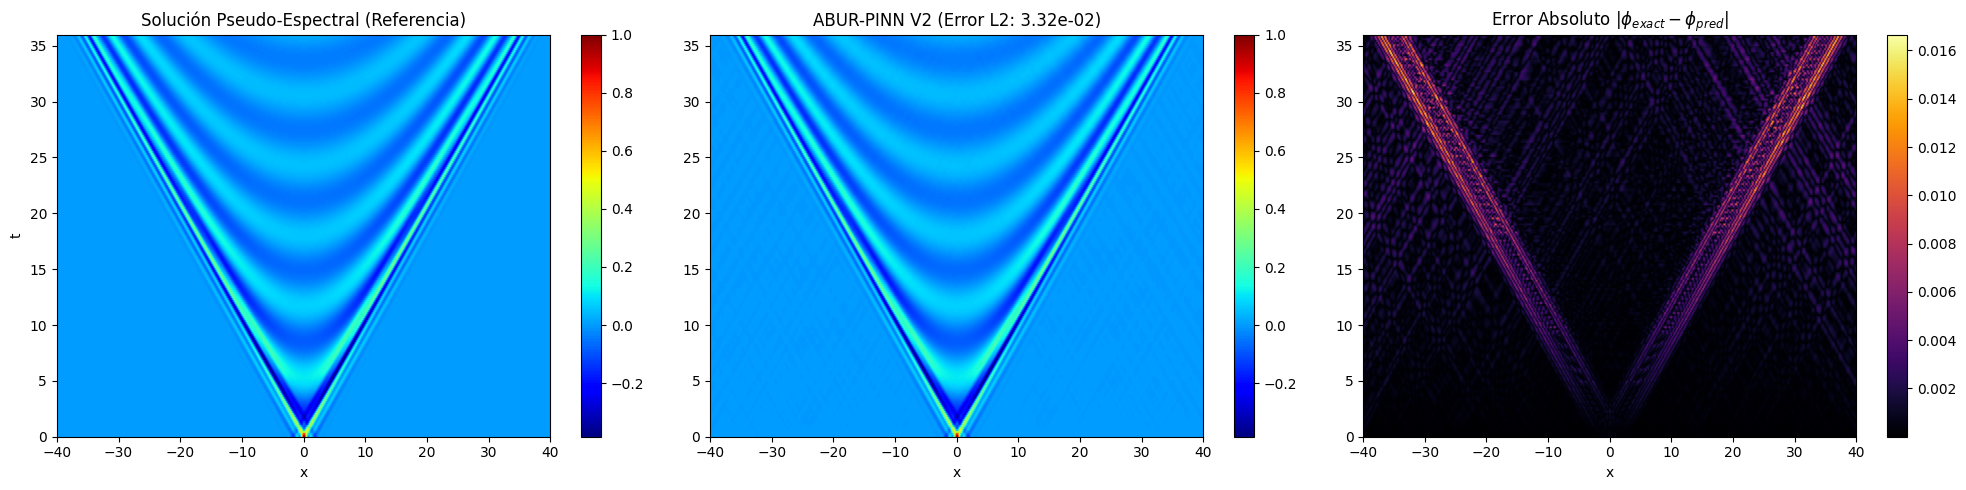
\includegraphics[width=\linewidth]{maburv2_sigma5_error.png}
  \caption[MABUR-PINN V2 with $\sigma=5$]{MABUR-PINN V2 with $\sigma=5$ (L2RE $3.32\%$): reference (left), prediction (center) and
  absolute error (right). The error is concentrated on the two fronts of the light cone.}
  \label{fig:exp2-sigma5}
\end{figure}
\verificar{in the first report this figure is under the heading ``V2 regularized''; check whether it
corresponds to $\sigma=5$ (its L2RE, $3.32\times10^{-2}$, matches $\sigma=5$)}

% =====================================================================
\section{Behavior of the Optimizer ADAM + LRA}\label{sec:exp-optimizer}
% =====================================================================

All the architectures were trained with ADAM and LRA to balance the terms of the composite loss. The final
losses (Table~\ref{tab:exp1-results}) show that MABUR-PINN V2 and AbuPINN reach the lowest values, followed by
M4-PINN and PINN-SIREN, while the vanilla PINN and MSF-PINN present higher losses (of order $10^{-5}$ and
$10^{-4}$), indicating difficulties to minimize simultaneously the PDE residual and the initial and
boundary conditions. The loss curves (Figure~\ref{fig:exp1-loss} and Appendix~\ref{app:figures}) show that:
\begin{itemize}
  \item ADAM + LRA reduces the total loss to orders between $10^{-7}$ and $10^{-5}$ after $10^{5}$
    epochs, but with noise due to the periodic readjustment of the weights $\lambda_i$;
  \item in AbuPINN, M4-PINN and MABUR-PINN the curves are more stable and the loss decreases rapidly,
    indicating a better balance of gradients; the total loss follows the physics loss, while the initial
    position loss decreases below $10^{-7}$;
  \item MSF-PINN shows high variance, probably because of its large number of parameters and the
    difficulty of training multi-scale embeddings.
\end{itemize}

\begin{figure}[htbp]
  \centering
  \begin{subfigure}[b]{0.49\linewidth}
    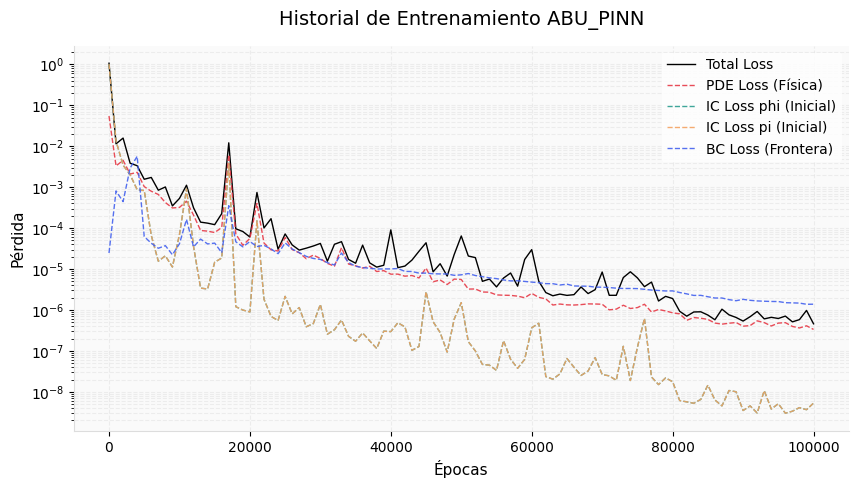
\includegraphics[width=\linewidth]{abu_loss.png}
    \caption{AbuPINN.}
  \end{subfigure}\hfill
  \begin{subfigure}[b]{0.49\linewidth}
    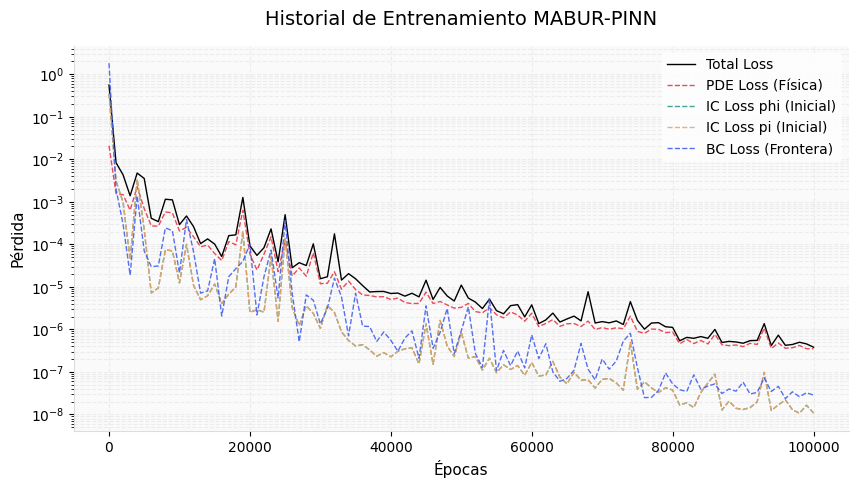
\includegraphics[width=\linewidth]{maburv2_loss.png}
    \caption{MABUR-PINN V2.}
  \end{subfigure}
  \caption{Training history (total, PDE, initial position, initial velocity and boundary losses).}
  \label{fig:exp1-loss}
\end{figure}

% =====================================================================
\section{Experiment 3: MABUR-PINN on the PINNacle Benchmark}\label{sec:exp-benchmark}
% =====================================================================

\paragraph{Methodology.}
To test whether the conclusions obtained for the Klein--Gordon equation extend to other classes of
PDEs, we adopted the experimental protocol of PINNacle \cite{hao2024pinnacle}. MABUR-PINN was evaluated
on a subset of $12$ tasks of the benchmark, covering elliptic (Poisson), parabolic (heat), hyperbolic
(wave) and nonlinear (Burgers, Navier--Stokes) equations in 1D and 2D (definitions in
Appendix~\ref{app:benchmark}). The results are compared against three representative methods of the benchmark:
LAAF, GAAF \cite{jagtap2020a,jagtap2020b} and FBPINN \cite{moseley2023}. Base configuration:
$5$ layers of $100$ neurons, $20\,000$ epochs, learning rate $10^{-3}$ (ADAM), $8\,192$ collocation points
and $2\,048$ boundary/initial points. LRA, causal training and Fourier embedding were \emph{not} used, in
order to adopt the experimental parameters of the benchmark. The branches of the softmax blend were chosen
for each family of PDEs (Table~\ref{tab:benchmark-activations}).

\begin{table}[htbp]
  \centering
  \caption[Branches of the softmax blend used for each PDE]{Branches of the softmax blend used for each PDE. $z=W\mathbf{x}+\mathbf{b}$ (dense branch, Glorot
  initialization); $z_s=\omega_0W_s\mathbf{x}$ (SIREN branch, $\omega_0=20$); output
  $=\sum_k\mathrm{softmax}(\bm\alpha)_k\sigma_k$.}
  \label{tab:benchmark-activations}
  \small
  \begin{tabularx}{\linewidth}{@{}llXc@{}}
    \toprule
    PDE & Variant & Branches & No. \\
    \midrule
    Burgers & 1d-C, 2d-C & $\sin(\beta_1z_s)$, $\tanh(\beta_2z)$, $1/(1+(\beta_3z)^2)$, $\ln(1+e^{\beta_4z})$, $e^{-(\beta_5z)^2}$ & 5 \\
    Poisson & 2d-C, 2d-CG, 2d-MS & $\ln(1+e^{\beta_1z})/\beta_1$, $z\,\sigma(\beta_2z)$ (Swish), $\tanh(\beta_3z)$, $1/(1+(\beta_4z)^2)$, $e^{-(\beta_5z)^2}$ & 5 \\
    Navier--Stokes & 2d-C & $\sin(\beta_1z_s)$, $\tanh(\beta_2z)$, $z\,\sigma(\beta_3z)$ (Swish), $e^{-(\beta_4z)^2}$ & 4 \\
    Wave & 1d-C & $\sin(z_s)$, $\cos(z_s)$, $\tanh(z)$, $1/(1+z^2)$ & 4 \\
    \bottomrule
  \end{tabularx}
\end{table}
\verificar{branches used for Heat, NS2d-CG, Wave2d-CG and Wave2d-MS}

\paragraph{Results.}
Table~\ref{tab:benchmark} shows the relative $L^2$ errors. MABUR-PINN obtains the best result in $8$ of the $12$
tasks: Burgers1d-C, Poisson2d-CG, Heat2d-MS, Heat2d-VC, NS2d-C, NS2d-CG, Wave1d-C and Wave2d-MS. LAAF is
the best in three tasks (Burgers2d-C, Poisson2d-MS, Heat2d-CG), FBPINN in Poisson2d-C and GAAF in
Wave2d-CG.

\begin{table}[htbp]
  \centering
  \caption[Relative $L^2$ error (L2RE) on the PINNacle benchmark]{Relative $L^2$ error (L2RE) on the PINNacle benchmark. In bold, the best result of each row.
  Data of LAAF, GAAF and FBPINN taken from Hao et al.~\cite[Table~3]{hao2024pinnacle}.}
  \label{tab:benchmark}
  \small
  \begin{tabular}{@{}llcccc@{}}
    \toprule
    PDE & Variant & LAAF & GAAF & FBPINN & MABUR-PINN \\
    \midrule
    \multirow{2}{*}{Burgers} & 1d-C & $1.43\times10^{-2}$ & $5.20\times10^{-2}$ & $2.32\times10^{-1}$ & $\mathbf{6.35\times10^{-3}}$ \\
                             & 2d-C & $\mathbf{2.77\times10^{-1}}$ & $2.95\times10^{-1}$ & -- & $4.67\times10^{-1}$ \\
    \midrule
    \multirow{3}{*}{Poisson} & 2d-C  & $7.68\times10^{-1}$ & $6.04\times10^{-1}$ & $\mathbf{4.49\times10^{-2}}$ & $6.03\times10^{-2}$ \\
                             & 2d-CG & $4.80\times10^{-1}$ & $8.71\times10^{-1}$ & $2.90\times10^{-2}$ & $\mathbf{2.98\times10^{-3}}$ \\
                             & 2d-MS & $\mathbf{5.93\times10^{-1}}$ & $9.31\times10^{-1}$ & $1.04$ & $1.32$ \\
    \midrule
    \multirow{3}{*}{Heat}    & 2d-CG & $\mathbf{2.39\times10^{-2}}$ & $4.61\times10^{-1}$ & $9.16\times10^{-2}$ & $3.71\times10^{-2}$ \\
                             & 2d-MS & $7.40\times10^{-2}$ & $9.85\times10^{-1}$ & $8.20\times10^{-2}$ & $\mathbf{1.87\times10^{-2}}$ \\
                             & 2d-VC & $6.42\times10^{-1}$ & $8.49\times10^{-1}$ & $9.52\times10^{-1}$ & $\mathbf{2.25\times10^{-1}}$ \\
    \midrule
    \multirow{2}{*}{Navier--Stokes} & 2d-C  & $3.60\times10^{-2}$ & $3.79\times10^{-2}$ & $8.45\times10^{-2}$ & $\mathbf{1.20\times10^{-2}}$ \\
                                    & 2d-CG & $8.24\times10^{-2}$ & $1.74\times10^{-1}$ & $8.27$ & $\mathbf{6.32\times10^{-2}}$ \\
    \midrule
    \multirow{3}{*}{Wave}    & 1d-C  & $4.54\times10^{-1}$ & $6.77\times10^{-1}$ & $5.91\times10^{-1}$ & $\mathbf{3.53\times10^{-1}}$ \\
                             & 2d-CG & $8.19\times10^{-1}$ & $\mathbf{7.94\times10^{-1}}$ & $1.06$ & $1.42$ \\
                             & 2d-MS & $1.06$ & $1.06$ & $1.03$ & $\mathbf{9.86\times10^{-1}}$ \\
    \bottomrule
  \end{tabular}
\end{table}
\verificar{whether the PINNacle values are means over several runs and how many runs were made for
MABUR-PINN}

\paragraph{Discussion by class.}
\begin{itemize}
  \item \textbf{Parabolic (heat).} MABUR-PINN is the best in the multi-scale and variable-coefficient
    problems, where the adaptive scales $\beta_i$ seem to help, and is second in the complex geometry
    (behind LAAF). Parabolic problems are, as expected from Table~\ref{tab:second-order}, the ones where the
    errors are smaller overall.
  \item \textbf{Elliptic (Poisson).} The results are mixed: the best result by one order of magnitude in
    the complex geometry (CG), second in the classic problem (C), and a failure (L2RE $>1$) in the
    multi-scale problem (MS), as for all the methods except LAAF.
  \item \textbf{Nonlinear (Burgers, Navier--Stokes).} MABUR-PINN is the best in three of the four tasks.
    Burgers2d-C, whose solution develops steep fronts, remains difficult.
  \item \textbf{Hyperbolic (wave).} This is the hardest class, as predicted in
    Section~\ref{sec:regularity-bridge}. MABUR-PINN is the best in Wave1d-C ($0.353$), but all the methods fail
    in the 2D tasks (L2RE between $0.79$ and $1.42$), and MABUR-PINN is the worst in Wave2d-CG (heterogeneous medium
    $c(\mathbf{x})$); the reason for this failure has not been analyzed yet. In Wave2d-MS the comparison is not informative, because, as shown
    in Section~\ref{sec:klein-gordon} and Appendix~\ref{app:benchmark}, its reference solution satisfies a Klein--Gordon
    equation with mass $2\pi^2$ instead of the stated wave equation; a network that minimizes the residual
    of the wave equation cannot approach that reference.
\end{itemize}

\paragraph{Threats to validity.}
The baselines are the published values of PINNacle and were not re-run by us; the branches of the
activation were chosen per family of PDEs, which is an additional degree of tuning that the baselines did
not have; and MABUR-PINN was run once per task. These three facts limit the strength of the comparison,
and they are addressed in the checklist of future work.

% =====================================================================
\section{Synthesis}\label{sec:exp-synthesis}
% =====================================================================

The experiments confirm, at least qualitatively, the three intuitions of Section~\ref{sec:regularity-bridge}.
First, smoothing helps the learner: the parabolic problems are the ones with the smallest errors, while the
hyperbolic ones (wave and Klein--Gordon) concentrate the failures, and inside the Klein--Gordon problem the
error of the best networks lives on the light-cone fronts, where the highest frequencies travel. Second, the
energy estimate of Theorem~\ref{thm:energy-estimate} explains why the derivative regularization did not help in a
periodic problem. Third, a small loss is not a small error: the preliminary experiment ($10^{-8}$ loss,
$9.5\%$ error) and PINN-SIREN show it clearly, as predicted by Theorem~\ref{thm:error-decomp}.

Regarding the proposed architecture, MABUR-PINN V2 obtained the lowest error on the Klein--Gordon equation and
the best result in $8$ of $12$ tasks of the benchmark. At the same time, the experiments show that the
Fourier embedding is still needed (V1 vs.\ V2) and that the scale $\sigma$ still matters
(Table~\ref{tab:exp2}); the adaptive activations reduce, but do not remove, this dependence. The bound
Equation~\eqref{eq:abu-bound} gives a theoretical reason for using bounded branches and a bounded range of scales,
which suggests replacing Swish, Softplus and exponential branches, and constraining $\beta_{\max}$, in
future versions.

\end{hyphenrules}
